\begin{figure}[H]
    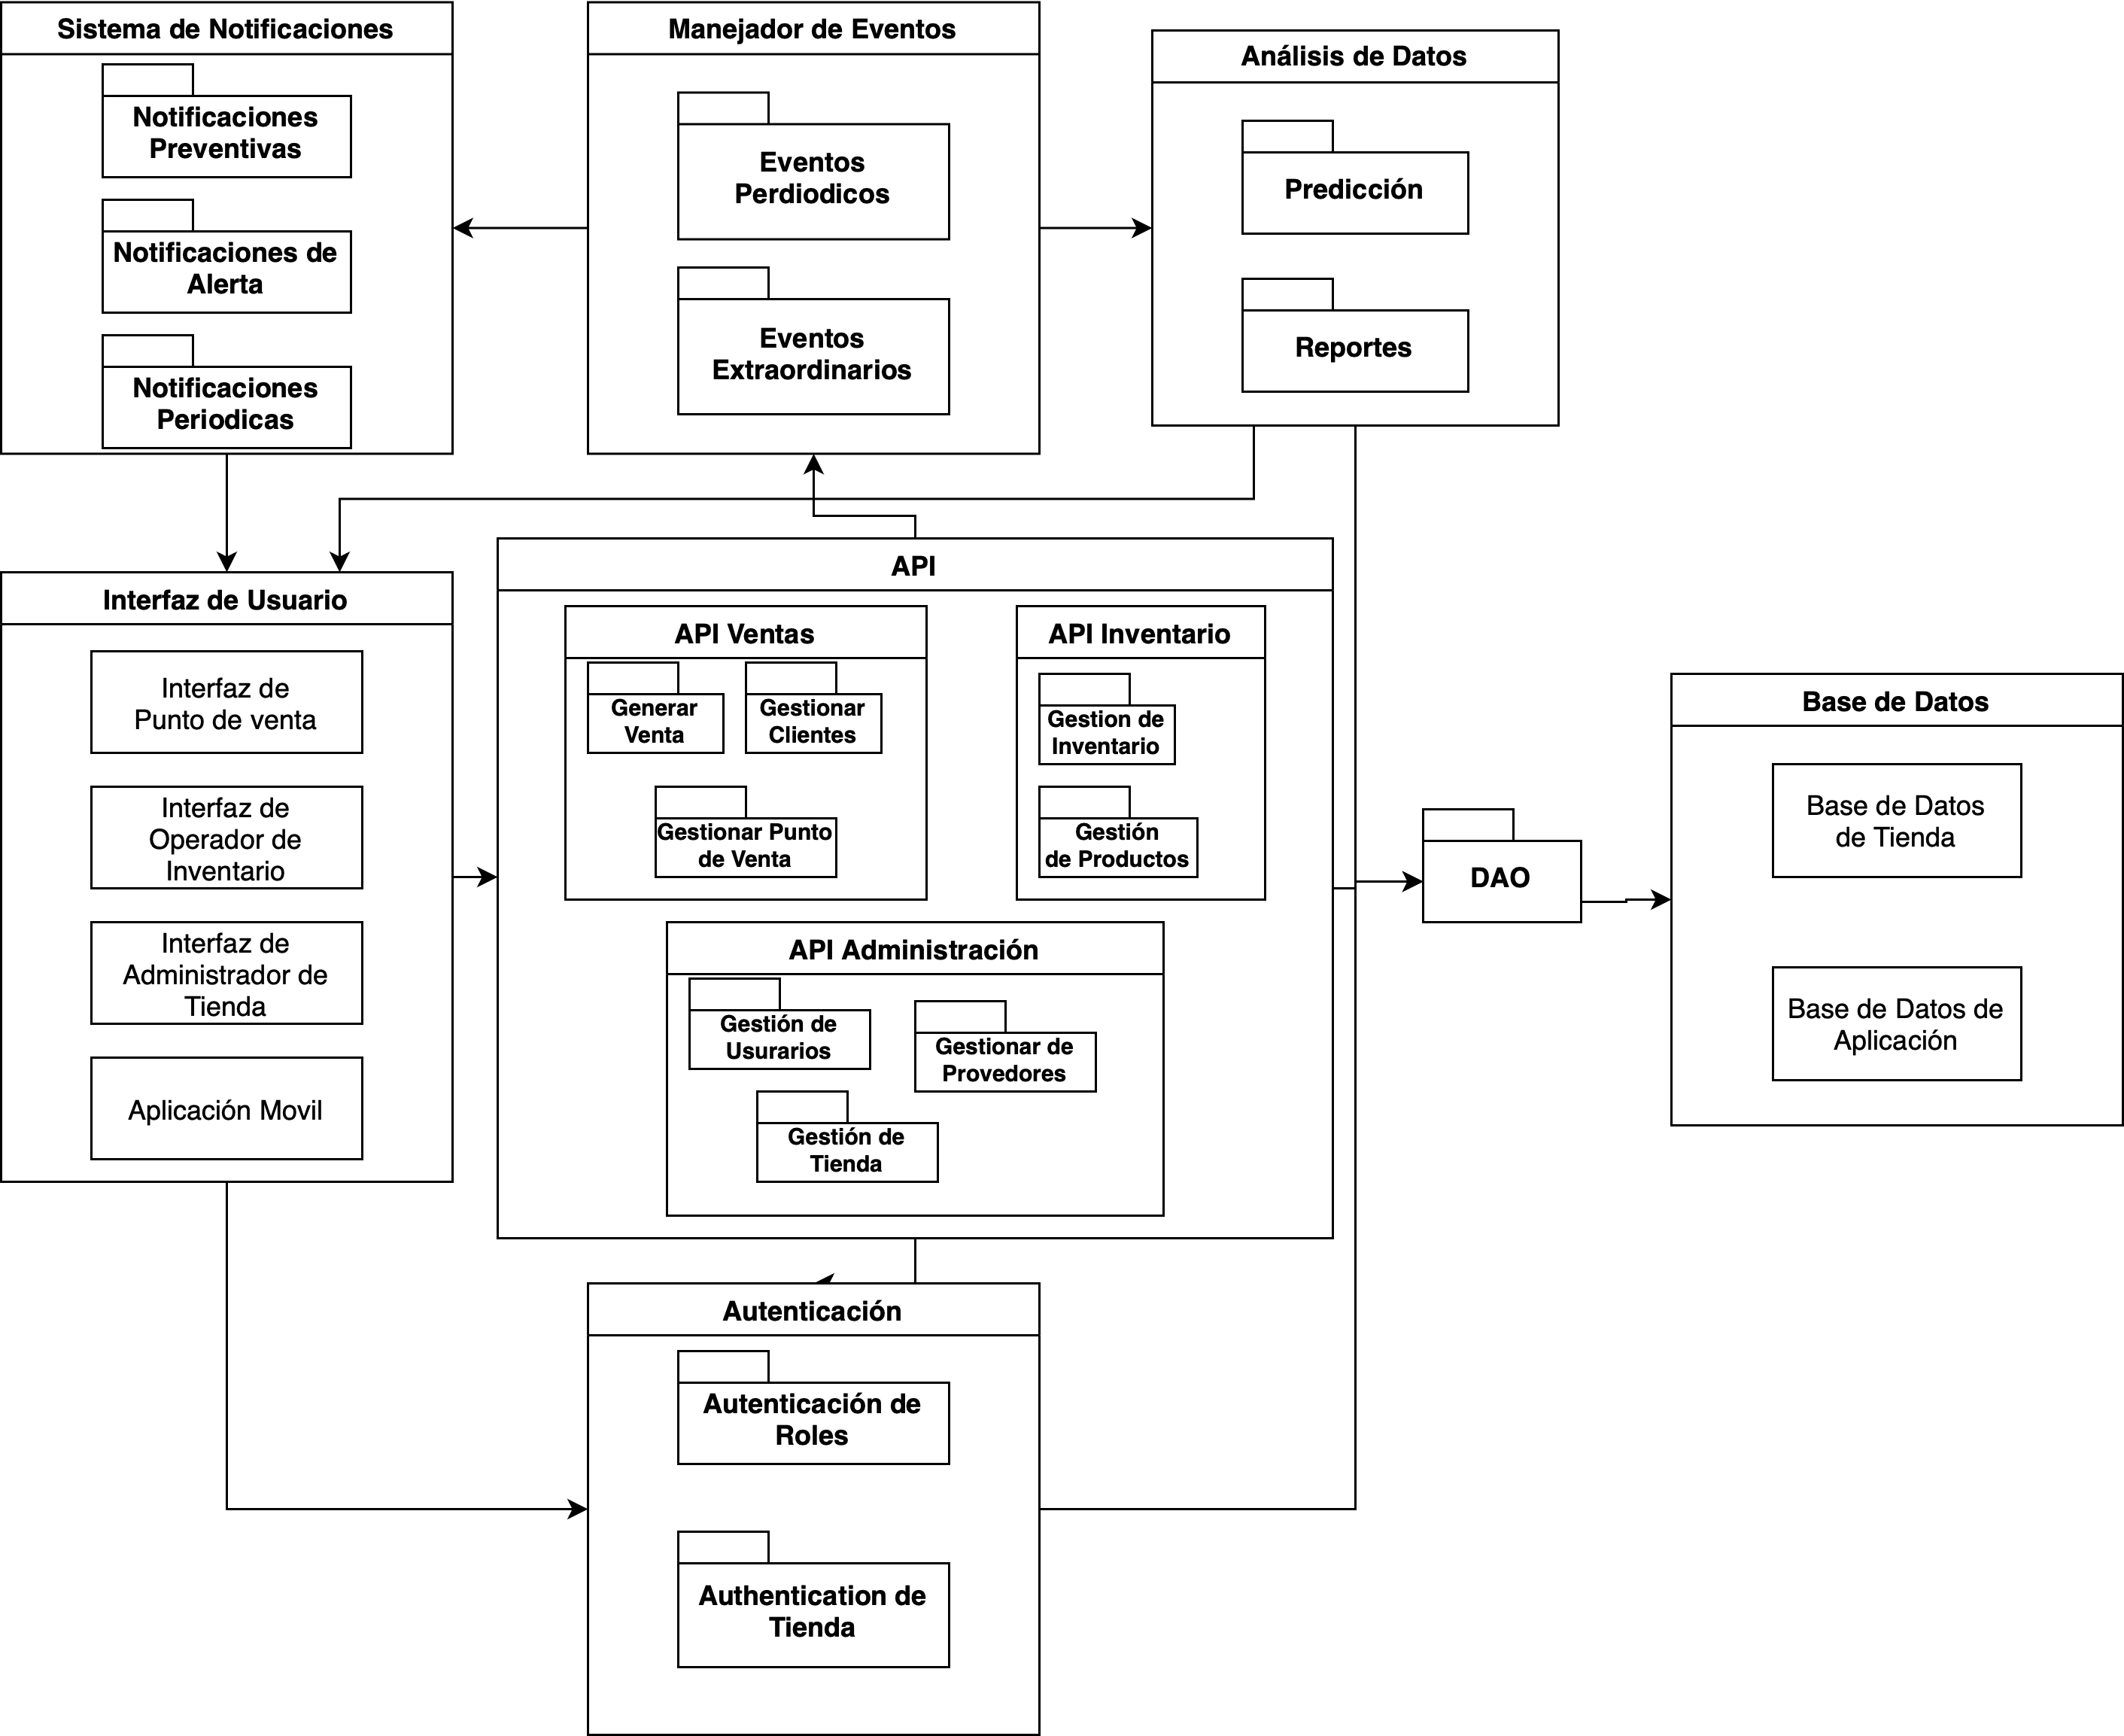
\includegraphics[width=\textwidth]{images/BackEnd.png}
    \centering
    \caption{Arquitectura del Backend de la Aplicación}
\end{figure}

\subsection{DAO}

El DAO (Data Access Object) será el encargado de administrar todos los accesos a la base de datos, permitiendo la 
interacción entre la aplicación y el almacenamiento de datos de manera estructurada y eficiente.

\subsection{API de Puntos de Venta}

Esta API gestionará las operaciones relacionadas con el punto de venta, permitiendo la generación de ventas, la administración 
de clientes y la gestión de los puntos de venta.

\subsubsection{Gestión de Venta}

Se encarga del procesamiento de ventas dentro del sistema, incluyendo la generación de tickets, 
cálculo de totales y aplicación de descuentos o promociones.

\subsubsection{Gestión de Clientes}

Administra la base de datos de clientes, permitiendo registrar información personal, historial de 
compras y preferencias para mejorar la experiencia del usuario.

\subsubsection{Gestión de Punto de Venta}

Coordina las operaciones en el punto de venta, integrando la administración de ventas, emisión de 
recibos y sincronización con el inventario para mantener un control actualizado de los productos vendidos.

\subsection{API de Operaciones de Inventario}

Encargada de administrar el inventario de la tienda, permitiendo el control de stock, registro de movimientos de productos y 
actualización de información de los artículos disponibles.

\subsubsection{Gestión de Inventario}

Controla el stock de productos, permitiendo realizar ajustes en las existencias, registrar 
movimientos y gestionar el abastecimiento de la tienda.

\subsubsection{Gestión de Productos}

Administra los productos disponibles en la tienda, permitiendo su creación, edición y 
categorización, así como la asignación de precios y descripciones.

\subsection{API de Administración de Inventario}

Facilita la gestión de productos y proveedores, asegurando el abastecimiento adecuado de la tienda y la correcta administración 
de los recursos.

\subsubsection{Gestión de Usuarios}

Permite administrar las cuentas de los usuarios del sistema, definiendo roles 
y permisos según su nivel de acceso dentro de la tienda.

\subsubsection{Gestión de Tienda}

Facilita la configuración y administración general de la tienda, incluyendo 
información comercial, ajustes operativos y personalización de la plataforma.

\subsubsection{Gestión de Proveedores}

Maneja la información de los proveedores, permitiendo registrar, actualizar y consultar 
datos de contacto, historial de compras y acuerdos comerciales.












\subsection{Manejador de Eventos}

El manejador de eventos procesará diversas acciones dentro del sistema, tales como ventas, asignaciones de tareas, eventos 
periódicos y recepciones de inventario. Su función principal es notificar a los módulos correspondientes, en especial al 
sistema de notificaciones.

\subsection{Sistema de Notificaciones}

El sistema de notificaciones será el encargado de enviar alertas y recordatorios a los destinatarios correspondientes 
según los eventos que lo activen. Dependiendo del tipo de evento, se generará una notificación específica.

\subsubsection{Notificaciones Periódicas}

Son aquellas notificaciones programadas por el administrador de la tienda para ser enviadas en intervalos regulares, 
conteniendo información relevante según la configuración establecida.

\subsubsection{Notificaciones Preventivas}

Notificaciones enviadas de manera anticipada en función de los eventos en curso dentro de la tienda, con el objetivo de 
prevenir posibles incidencias o tomar decisiones estratégicas a tiempo.

\subsubsection{Notificaciones de Alerta}

Se generan ante eventos extraordinarios o críticos que ocurran en la tienda. Estas alertas son enviadas de forma 
inmediata a los usuarios correspondientes para su pronta atención.

\subsection{Análisis de Datos}

Este módulo se encargará del procesamiento y análisis inteligente de la información disponible en el sistema, permitiendo 
obtener conocimientos útiles a partir de los datos almacenados.

\subsubsection{Pronósticos}

Proveerá predicciones sobre eventos futuros con base en datos históricos, buscando ofrecer resultados 
lo más precisos posible.

\subsubsection{Reportes}

Generará informes personalizados según los datos requeridos por el usuario, extrayendo y procesando la 
información relevante de la base de datos.

\subsection{Autenticación}

Este módulo verificará la identidad de los usuarios y validará sus permisos para acceder a funciones 
específicas dentro del sistema.

\subsubsection{Autenticación de Roles}

Validará las acciones que un usuario puede realizar dentro de una tienda específica, asegurando 
que solo accedan a las funcionalidades autorizadas.

\subsubsection{Autenticación de Tienda}

Se encargará de validar el acceso a una tienda determinada, asegurando que el usuario tenga los permisos 
necesarios para ingresar a la misma.
